\entry{Semana de 16/06/2025.} 
\section{Miércoles 18/06/2025.}

\subsection*{Notas del día.}
\begin{itemize}
	\item Efectivamente cambia tener la resistencia tierra o no. A tierra la resonancia es como 72kHz y sino es como 60.260 kHz. 
	\item Dispositivo en el aire da resonancia en 53.190 aproximadamente. 
	\item Estaba tratando de medir con el generador apagado. 
	\item Tomé medición nuevo\_frozado.bin con f=52.60 kHz y parece ser coherente con lo de ates.
	\item Creo que a lo de tiempo real no le da la relocuión temporal. 
	\item Voy a cambiar la resitencia por una menor. 
	\item Puse una de supuestamente 10 $\Omega$. Aumenta bastante el ruido. Por ahí era 10 k$\Omega$. 
	\item Puse ahora una de 360 $\Omega$. Ahora es 52.905(37) kHz la resonancia aprox. No sé si cambia mucho, parece que teine menos ruido en general.  
	\item Pyqtgraph funciona bien en tiempo real, un punto por 0.015 segundos, mientras que matplotlib pone uno por 0.15 más o menos. Cambió el backend de matplotlib.
	\item Volví a la rsistencia de 1.8 k$\Omega$ y ahora 3.5 cm de altura y resonancia 52.667 kHz. ara estos rotar\_caja.bin. Idea de rotarla al moverlo por accidente.
	\item Ahora 52.685 kHz rotar\_caja2.bin. Se excitaron más modos, pero poca amplitud y más ruido, tal vez media móvil.
	\item Dos gotas con jeringa. 
	\item Ahora con 10$\Omega$ confirmado con multímetro rotar\_caja. 
	
	\item Ahora agua de la canilla 1.8k$\Omega$, 4.3 cm de altura y 51.339 (1) kHz de resonancia. 
	\item Ahora agua de la canilla y 9k$\Omega$. 50.525 kHz.
	
	\item Ahora 100pF de capacitancia y 1.8 k$\Omega$ al rotar la caja. 67.911 kHz sumergido. "100pF.bin". 
	
	\item Ahora 47pF y 1.8 k$\Omega$ al rotar la caja. 71.551 kHz. No sé si está cambiando mucho. 
	
	\item Ahora 10nF y 1.8k$\Omega$ al rotar la caja. 17.047 kHz. Ahora sí es puro ruido. 
	
	\item Ahora 1pF y 1.8 k$\Omega$ al rotar la caja. No parecía funcionar (¿resonancia a 1kHz?). 
	
	\item Ahora 10pF resonancia 74.253 kHz parece que nos limita a eso la capacitancia del sensor sumergido.  
	
	\item Voy a hacer la calibración con los valores de siempre, 560pF y 1.8 k$\Omega$. 51.428 kHz. $\Omega$. M e olvidé de poner fase 0°, lo dejo en la carpeta sin 0.. 
	. de nuevo ahora sí, f=52.344 kHz. Da bastante lineal con poco error con cuorte de 1.000 kHz. 
\end{itemize}

\vspace{2em}
\subsection*{Visualización en tiempo real.}
Estuve trabajando en la implementación de la visualización en tiempo real. Primero intenté con matplotlib pero solo llegaba a graficar como mucho 10 puntos por segundo. Después de timear todo me di cuenta de que la adquisición y procesado daba para mucho más que eso entonces debía ser matplotlib que tardaba en plottear los nuevos puntos. 


\begin{figure}[!ht] %  
	\centering
	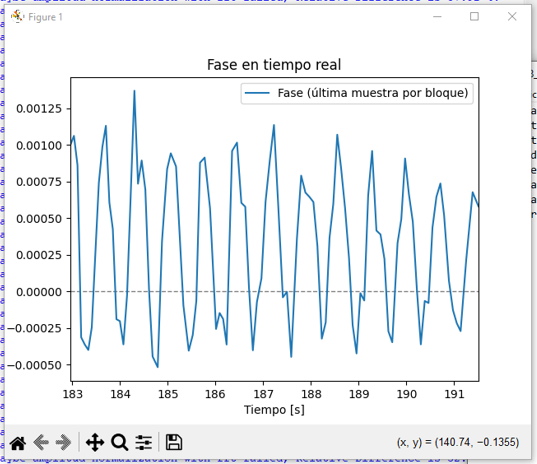
\includegraphics[width=0.567\linewidth]{Figures/16_06_2025/Tiempo_real_matplotlib}
	\caption{Medición en tiempo real usando matplotlib.}
	\label{fig:tiemporealmatplotlib}
\end{figure}

Después traduje el código mediante ChatGPT para usar pyQTGraph y ahí si empezó a funcionar bastante mejor llegando hasta unos 50 puntos por segundo. 



La forma en que funciona esto es la siguiente. Tengo la adquisición contínua configurada (sin guardar en archivo pero con buffer circular). La placa manda de mínimo de a 8192 puntos en este modo con lo cual puse un buffer de este tamaño, y en el bucle principal cada vez que la placa manda estos scans se analizan con el lockin con el método elegido y se promedian los últimos puntos de la fase, que es lo que se grafica. 

\begin{figure}[th!]
	\centering
	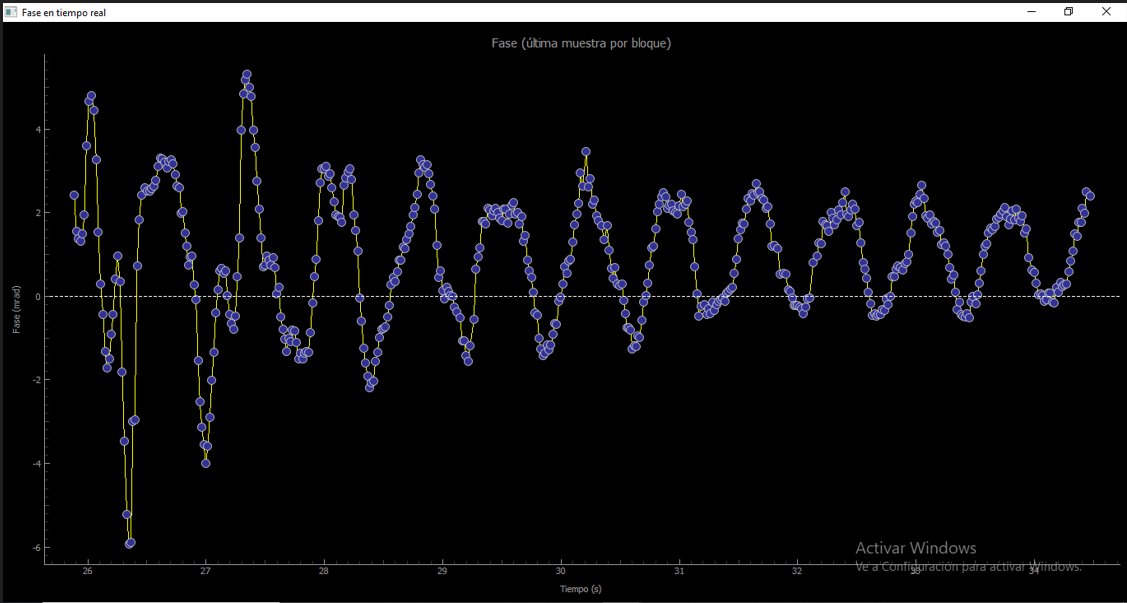
\includegraphics[width=0.7\linewidth]{Figures/16_06_2025/Tiempo_real_pyqtgraph}
	\caption{Gráfico en tiempo real con pyQTGraph.}
	\label{fig:tiemporealpyqtgraph}
\end{figure}


Se podrían usar buffers más grandes pero habría que tomar solo la tira de puntos nueva según la total que hay mandado usando módulo o algo así.  

Al siempre reempezar el análisis en cada iteración hay más ruido, habría que probar ir guardando los últimos puntos del filtro exponencial y empezar la iteración siguiente con los finales de la anterior, así además se podrían poner todos los puntos (o algún resampleo) en vez de uno solo para evitar las cosas que hace al inicio del análisis.

\subsection*{Modos de la caja.}
Estuve probando otras formas de excitar más modos de la caja que solo el fundamental con el forzado longitudinal. Lo que probé fue darle una rotación súbita y los resultados fueron los siguientes:

\begin{figure}[th!]
	\centering
	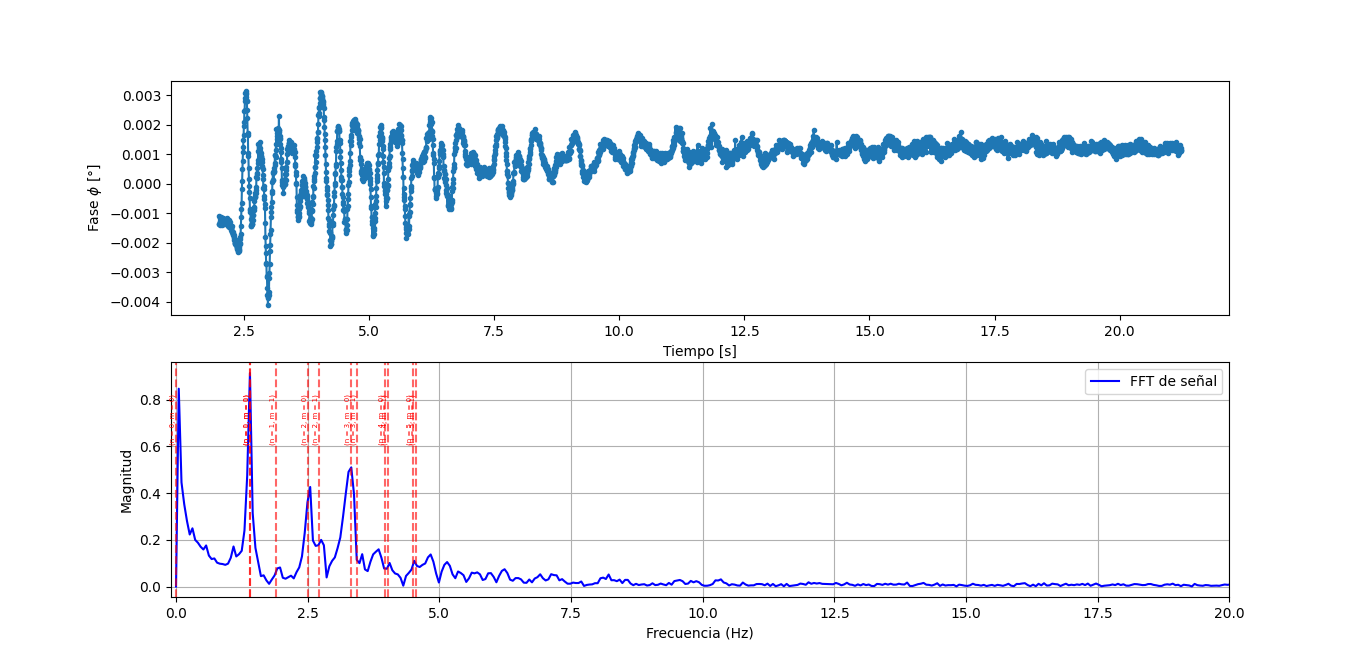
\includegraphics[width=0.87\linewidth]{Figures/16_06_2025/Rotas_caja}
	\caption{Espectro de la respuesta de la cuba al rotarla súbitamente.}
	\label{fig:rotascaja}
\end{figure}

Se nota claramente la excitación de varios de los primeros modos. Hacia el final hay más ruido, puede ser por la baja amplitud de las ondas, que no estaba centrado o que justo esa zona del alambre sumergido no era l más recta. Parte del mismo se puede sacar disminuyendo la frecuencia de corte (ahí es 1kHz). 


\subsection*{Agua de la canilla.}
Después probé hacer mediciones con agua de la canilla y no parece haber diferencias significativas con el agua destilada. Más abajo la calibración que es dentro de todo lineal, más allá de lo que supongo son las irregularidades del alambre.

\begin{figure}[th!]
	\centering
	\includegraphics[width=0.78\linewidth]{Figures/16_06_2025/Calibración_canilla}
	\caption{Calibración de fase contra altura para agua de la canilla.}
	\label{fig:calibracioncanilla}
\end{figure}

Los parámetros del ajuste fueron: $R^2=0.99555$,	$\chi_\nu^2=18.67689$,	pendiente $m = (0.00143 \pm 0.00002)\; mm/°$,	e intercept $b = (-0.00145 \pm 0.00009)\; mm$. 

Después, alguna medición de ejemplo tenemos: 
\begin{figure}[th!]
	\centering
	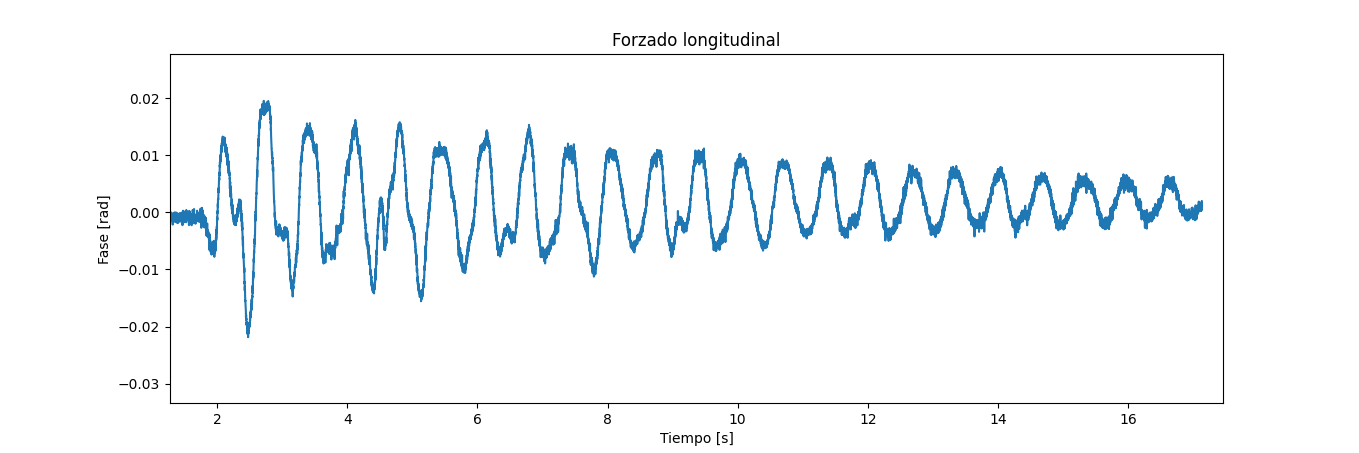
\includegraphics[width=0.87\linewidth]{Figures/16_06_2025/Forzado_canilla}
	
	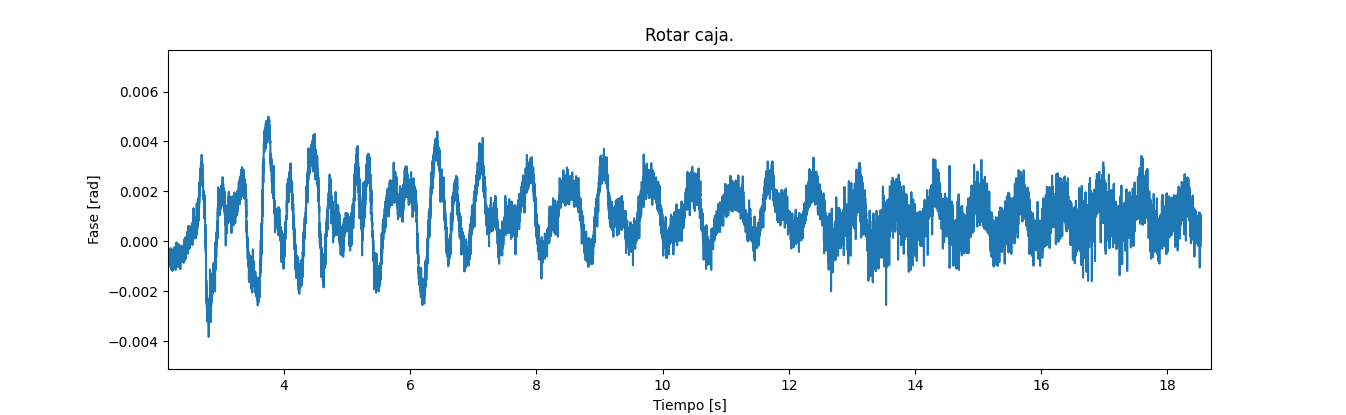
\includegraphics[width=0.87\linewidth]{Figures/16_06_2025/Rotar_caja_canilla}
	\caption{Algunas mediciones de prueba con agua de la canilla.}
	\label{fig:forzadocanilla}
\end{figure}




\subsection*{Variar parámetros del sistema.}
Para intentar aumentar el rango de la fase y disminuir el error al medir amplitudes chicas intenté disminuir la resistencia o la capacitancia para aumentar el factor de calidad que va multiplicando al $\Delta l$ pero en general no hubo muchos cambios. 

\begin{figure}[th!]
	\centering
	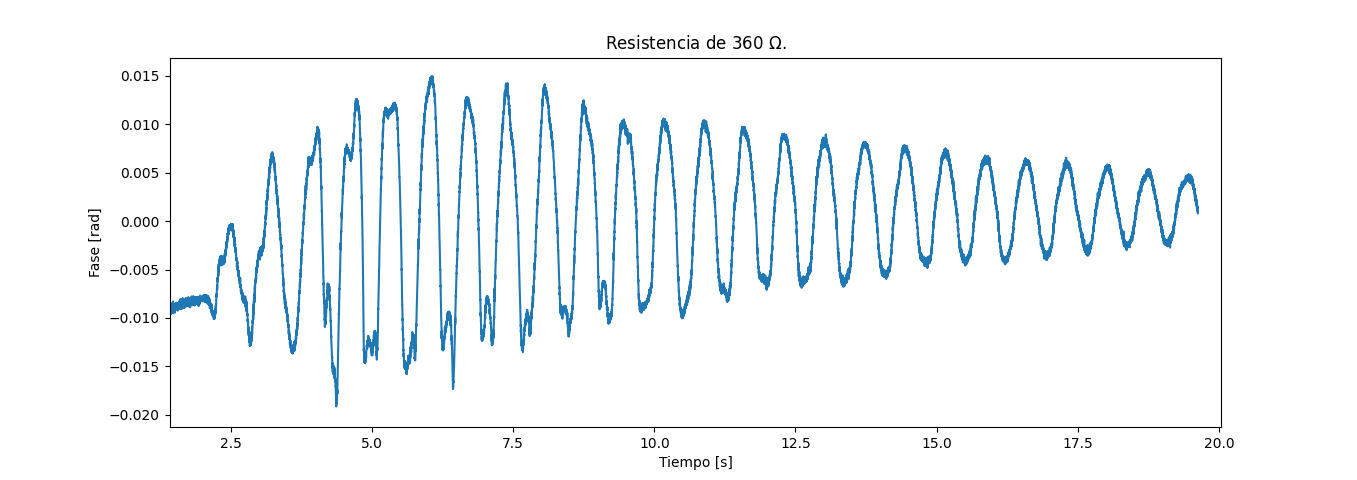
\includegraphics[width=0.678\linewidth]{Figures/16_06_2025/Forzado_360Ohm.png}
	
	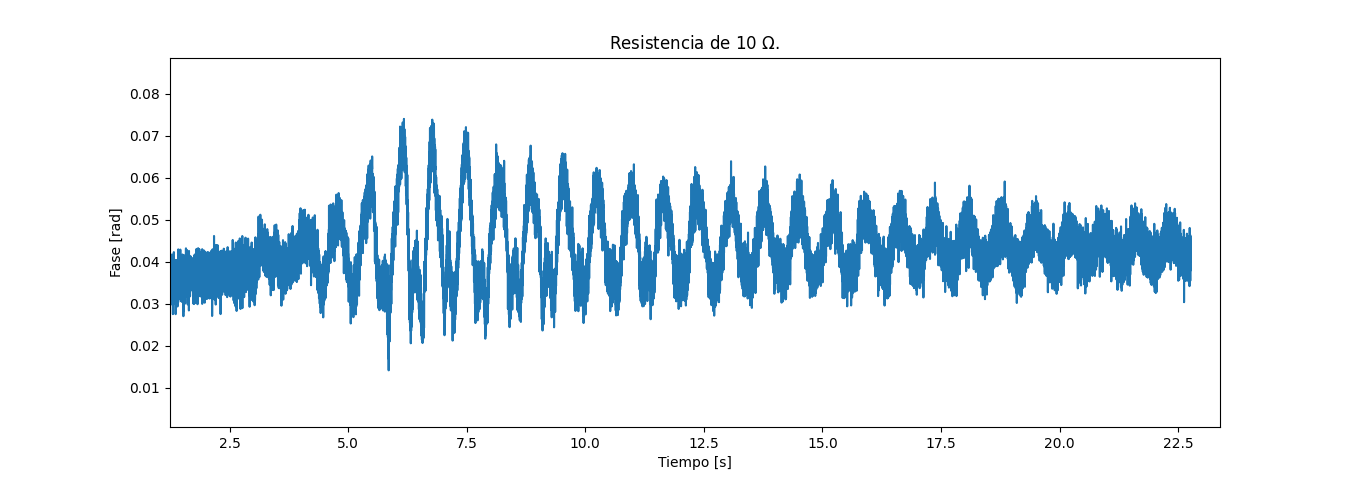
\includegraphics[width=0.678\linewidth]{Figures/16_06_2025/Forzado_10Ohm.png}
	\caption{Algunas mediciones de prueba con distintas resistencias.}
	\label{fig:resistencias}
\end{figure}

En cualquier caso parece que hay más ruido con 10 $\Omega$ que con las más altas, por ahí estaba rara la resistencia pero la probé con el multímetro y marcaba 10 $\Omega$. Aunque parece que sí llegó a extender algo el rango, habría que probar ma´s con esto, o cambiando a esta resistencia y otro capacitor, tal vez muy baja comparada con las otras impedancias y caía poco el voltaje y habría que usar gain. Efectivamente!!! la amplitud máxima es de 0.025 V comparada con la del canal de referencia de 2.5 V, habría que usar gain x10 o más Para la de $360$ $\Omega$ la amplitud máxima era de $0.6799$.  Usar gain analógico aparte tal vez.

Respecto a la capacitancia solo se puede bajar hasta cierto punto ya que luego de este empieza a ganar la $C_{eq}$ del alambre sumergido en la altura de equilibrio, con una frecuencia máxima de unos 72 kHz. Respecto a la resistencia no noté mucha diferencia, sí que al aumentarla aumenta el ruido hasta que para 100 $k\Omega$ es solo eso, pero nada al bajarla, por ahí hay una resistencia ganándole en otro lado, como la placa. 

Con este nivel de ruido creo que no llega a medir la amplitud de las ondas generadas al dejar caer una gota de agua. Queda aumentar la inductancia, que es complicado, o modificar la relación $r/e$ del alambre de cobre, pero para eso habría que comprar otro, ya que queremos ya sea disminuir el coating o aumentar el radio. Tal vez probar el alambre de acero con el esmalte en aerosol. % cobre.  

\section{Canal de la Facultad de Ingeniería (Paseo Colón).}
Fuimos con Pablo y Lucía N. a visitar el canal de la Facultad de Ingeniería de la UBA, con la idea de más adelante realizar experiencias con el sensor en éste. 

El canal de 72 metros se encuentra debajo de las escalinatas casi a nivel del suelo. Tiene 2 metros de profundidad y unos 5 metros de ancho. El agua que tiene es de la canilla, trajimos una botellita (que antes tenía agua destilada) llena para hacer pruebas con el sensor por la salinidad. 

Una vez por año se vacía y se cambia el agua, debería tener pocas cosas agregadas, solo algo de cloro. Notamos algunos pedazos del cielo raso que se había desprendido y caído dentro del canal pero nada más que eso. Como el sensor funcionó con el agua de la canilla de Ciudad esperaríamos que también lo haga con esta. 

En uno de los extremos el canal tiene un shaker del ancho del canal para generar olas, siendo efectivamente un sistema 1D. Las olas se generan con períodos de 0.5, 1 o 2 segundos y se podrían llegar a hacer solo pulsos apagando y prendiéndolo rápidamente. Llegan al extremo opuesto del canal con una amplitud de unos 10 cm. 

\begin{figure}[!ht]
	\begin{minipage}[c]{0.5\textwidth}
			\begin{subfigure}{\textwidth}
					\centering
					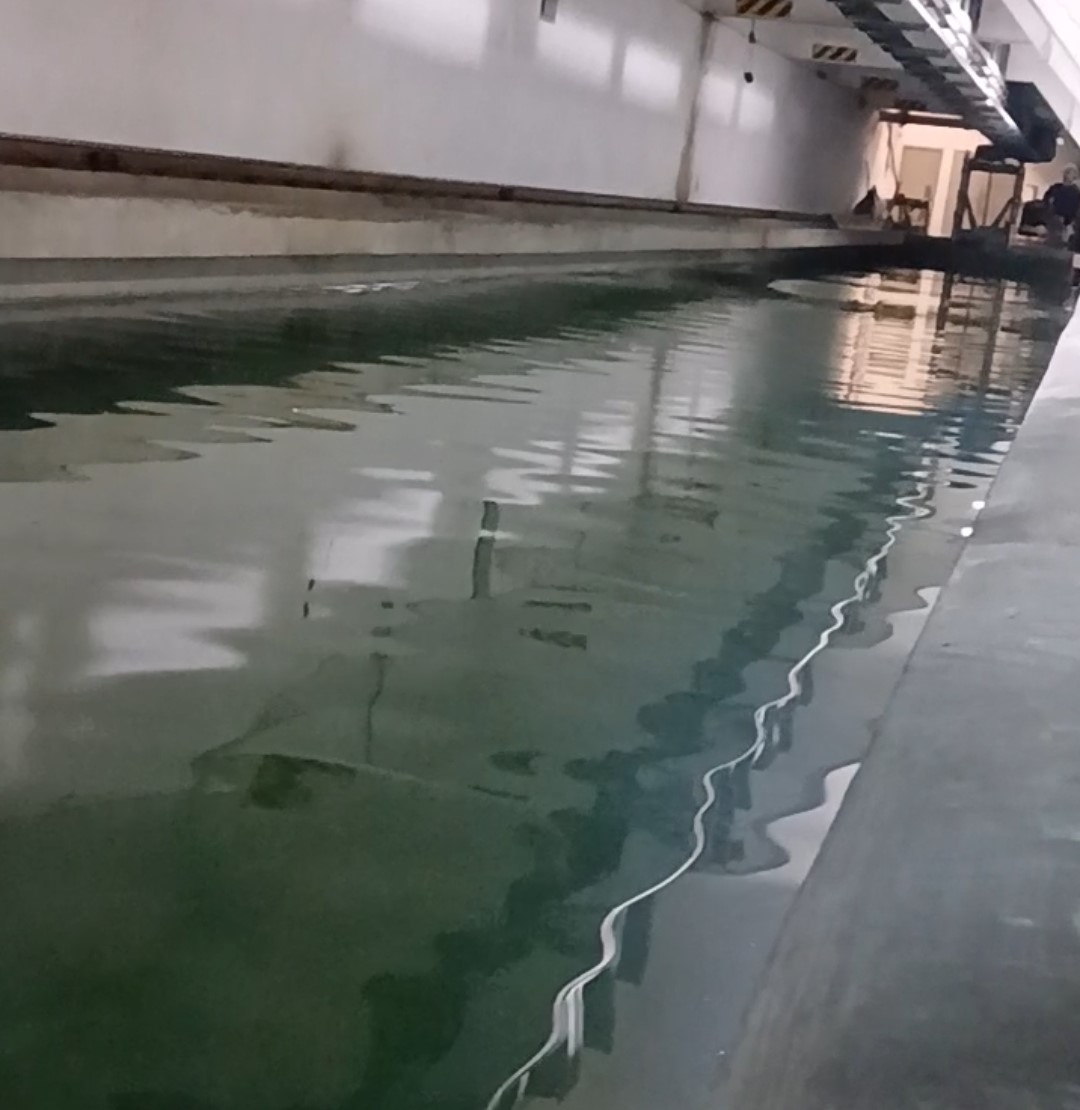
\includegraphics[width=0.8\textwidth]{Figures/16_06_2025/Shaker.jpg}
					\captionsetup{width=0.8\textwidth}
					\subcaption{}
				\end{subfigure}
		\end{minipage}\begin{minipage}[c]{0.49\textwidth}
			\begin{subfigure}{\textwidth}
					\centering
					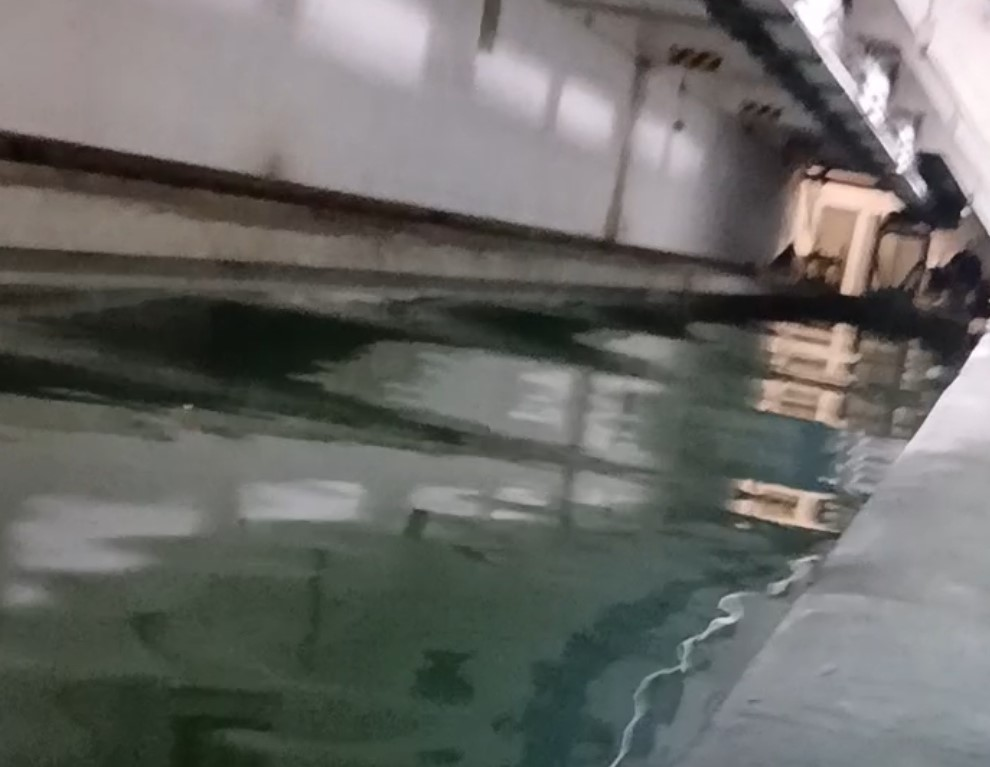
\includegraphics[width=0.98\textwidth]{Figures/16_06_2025/Olas.jpg}
					\captionsetup{width=0.8\textwidth}
					\subcaption{}
				\end{subfigure}
		\end{minipage}
	\caption{Shaker al inicio del canal, con y sin olas.}
	\label{fig:shaker}
\end{figure}

En el extremo opuesta hay un absorvedor de tablas de madera. Como no hay alguno otro más sofisticado nos comentaron que entre ensayo y ensayo hay que esperar un rato para que se vuelva a calmar el agua.

\begin{figure}[th!]
	\centering
	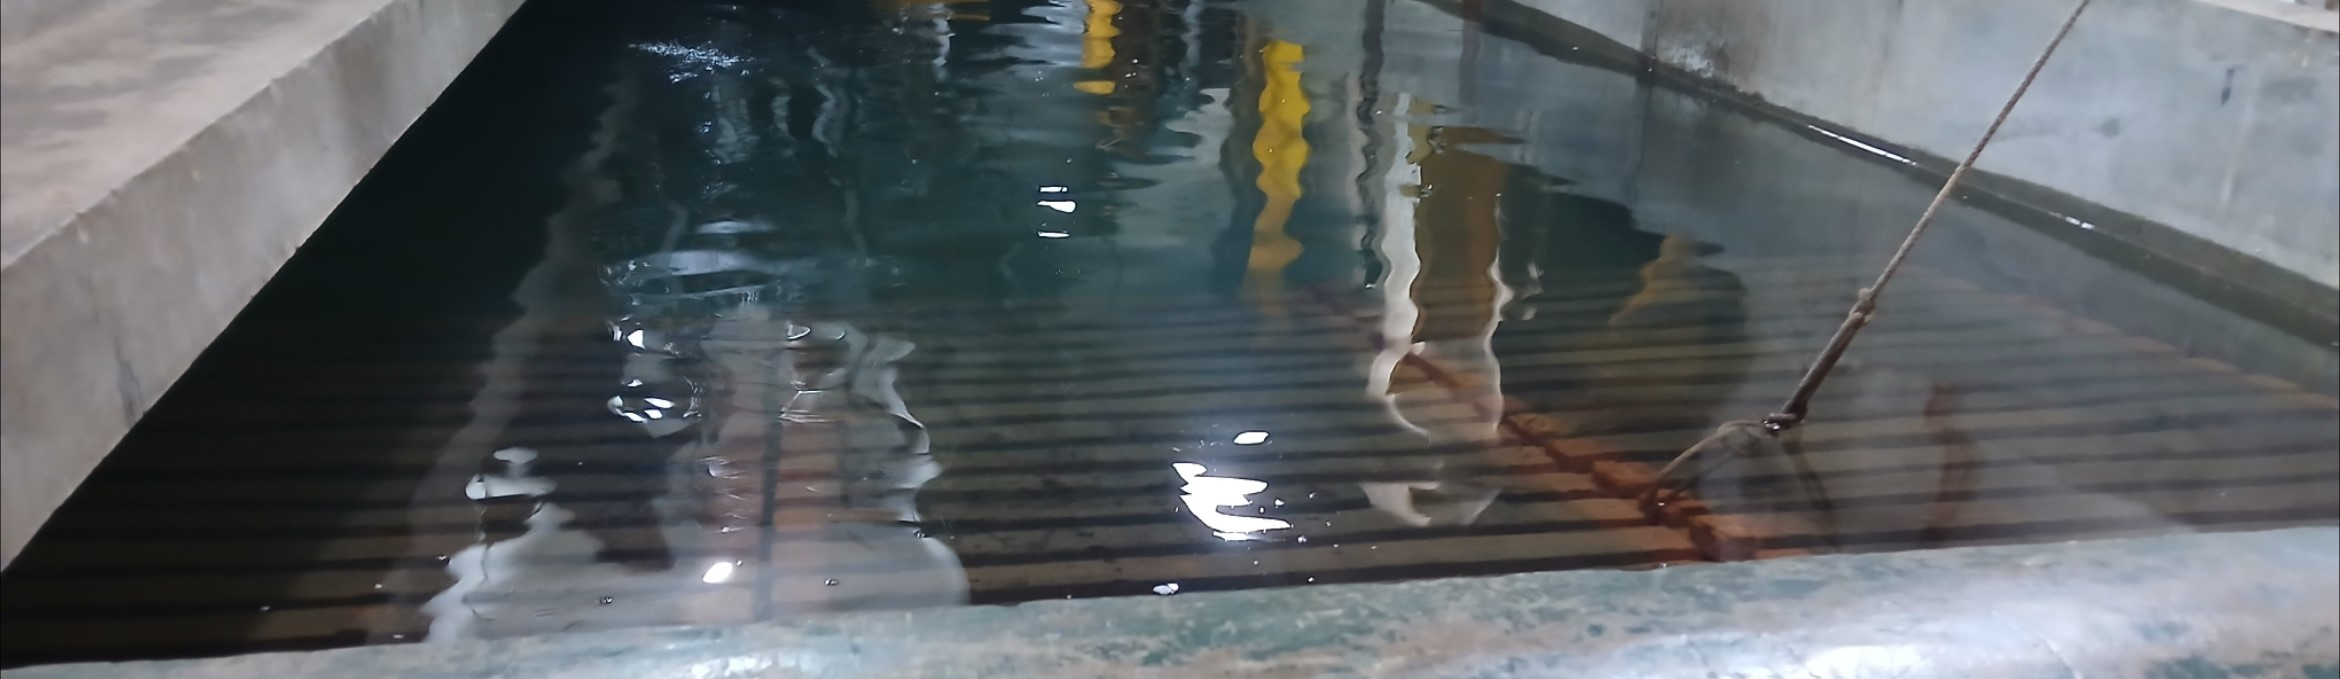
\includegraphics[width=0.7\linewidth]{Figures/16_06_2025/breakrer}
	\caption{Rompeolas del final del cananl.}
	\label{fig:breakrer}
\end{figure}


Por arriba hay un carrito que se desplaza a lo largo del canal con los operarios arriba y permite transportar barcos modelo a escala (equipados con un dinamómetro) para realizar distintas pruebas, ya sea con el agua calma o con olas del shaker. Los barcos a modelo se fabrican ahí mismo a mano. Se tallan sobre bloques de parafina (antes se usaba madera tratada) las líneas de agua de un plano con una fresadora que va siguiendo el trazado del operario. Luego la forma escalonada se lija y se hace un molde sobre el cual se hace el modelo final creo que con fibra de vidrio y ya pintado. 

\begin{figure}[!ht]
	\begin{minipage}[c]{0.5\textwidth}
			\begin{subfigure}{\textwidth}
					\centering
					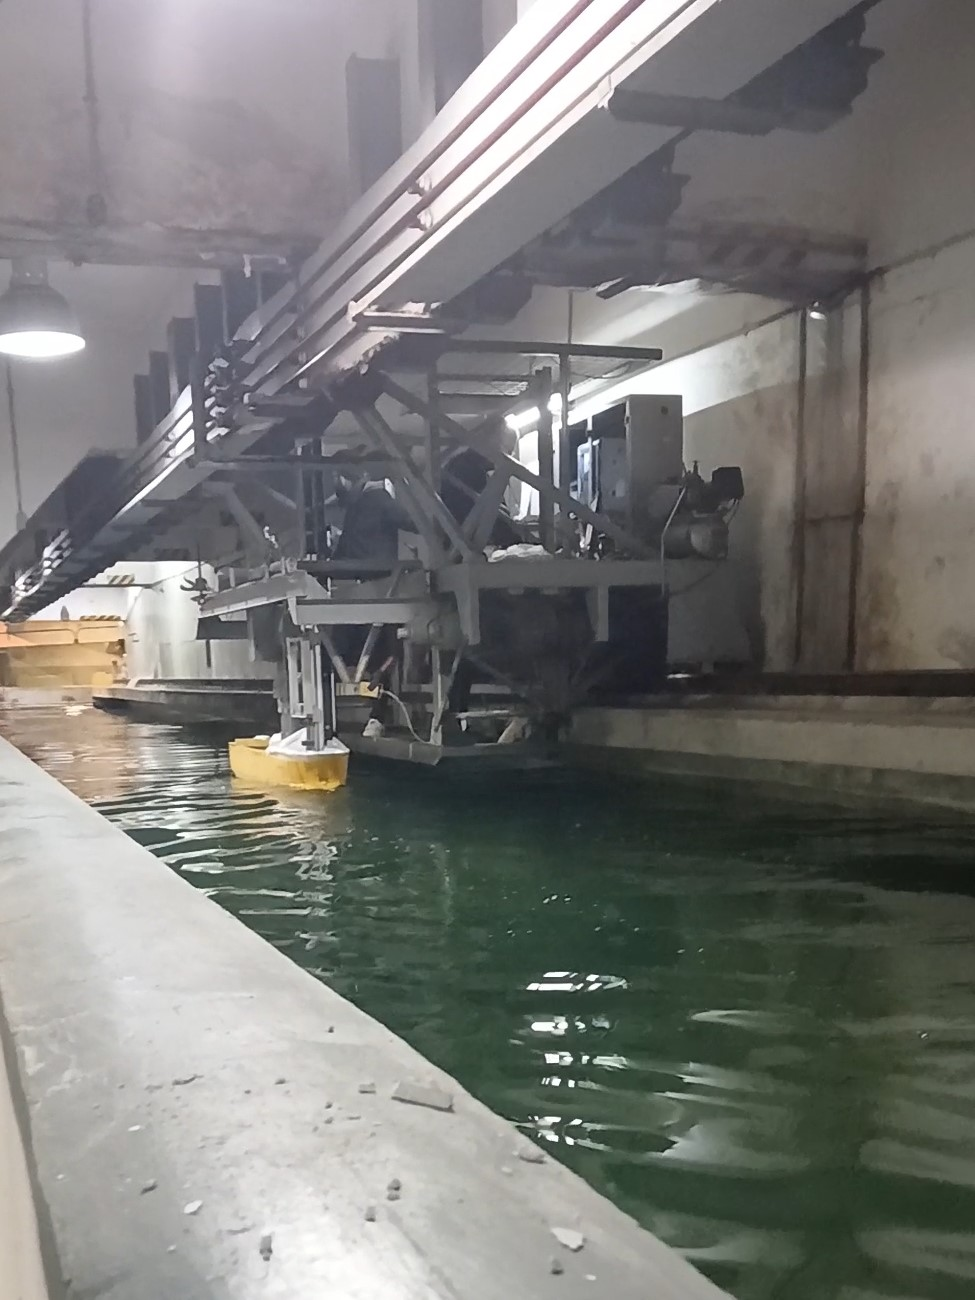
\includegraphics[width=0.68\textwidth]{Figures/16_06_2025/Carro.jpg}
					\captionsetup{width=0.8\textwidth}
					\subcaption{}
				\end{subfigure}
		\end{minipage}\begin{minipage}[c]{0.49\textwidth}
			\begin{subfigure}{\textwidth}
					\centering
					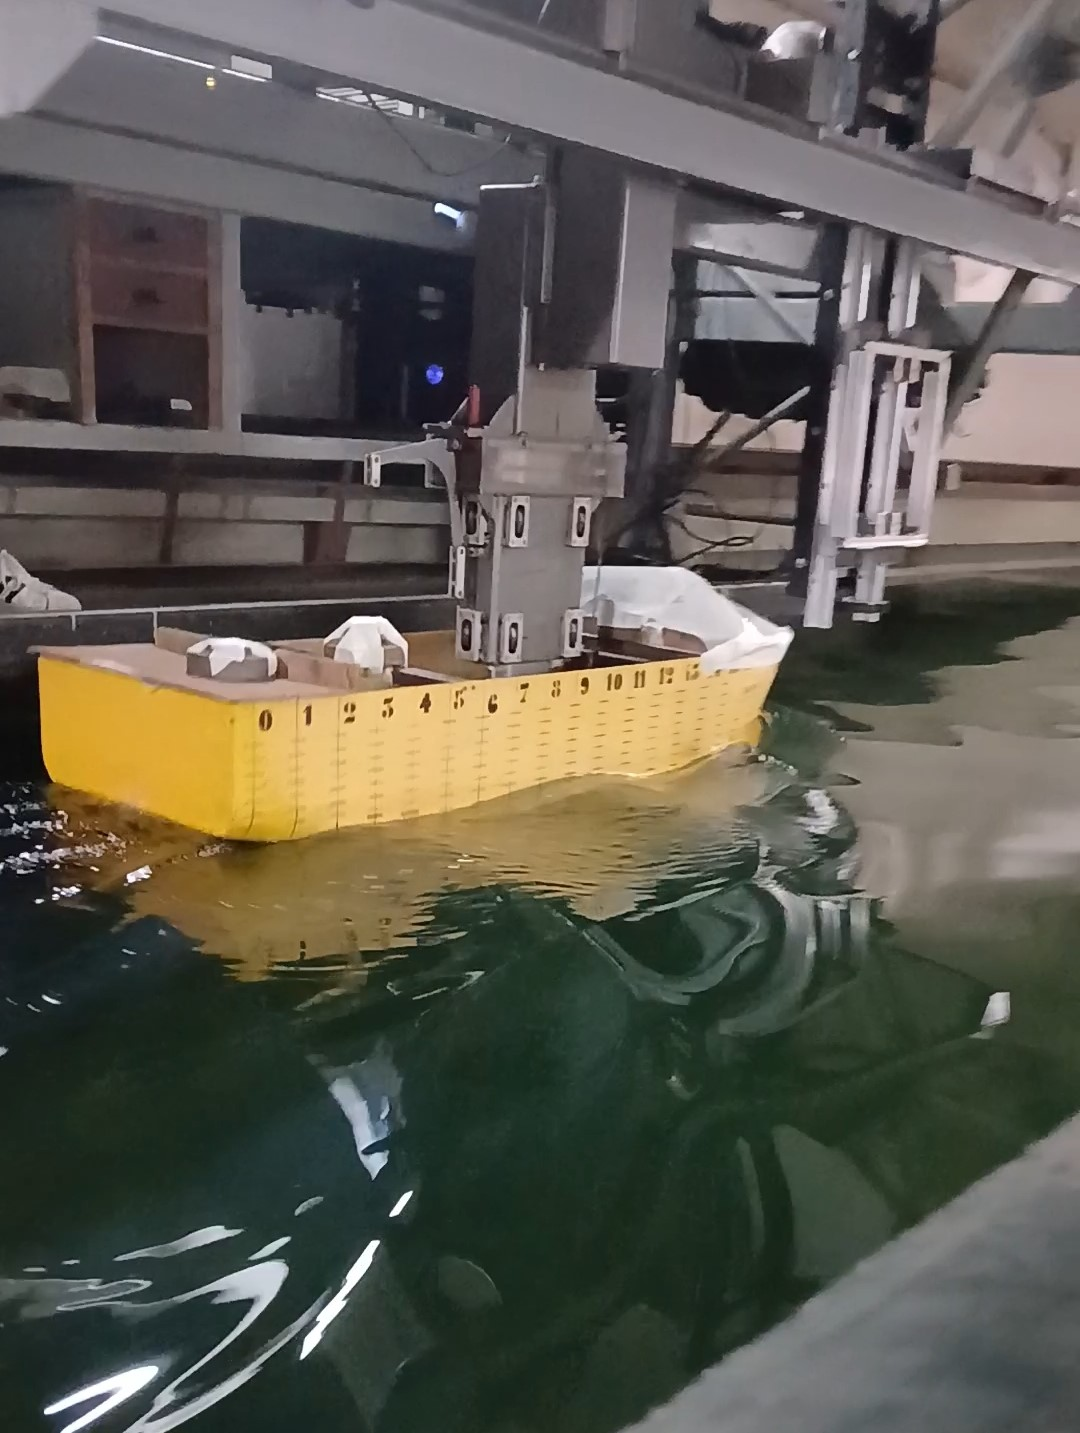
\includegraphics[width=0.68\textwidth]{Figures/16_06_2025/Barco.jpg}
					\captionsetup{width=0.8\textwidth}
					\subcaption{}
				\end{subfigure}
		\end{minipage}
	\caption{Carro que se desplaza sobre el canal con el barco modelo a escala.}
	\label{fig:barco}
\end{figure}

El canal cuenta con dos ventanas en las cuales se puede filmar el perfil del agua. % , n 

\begin{figure}[th!]
	\centering
	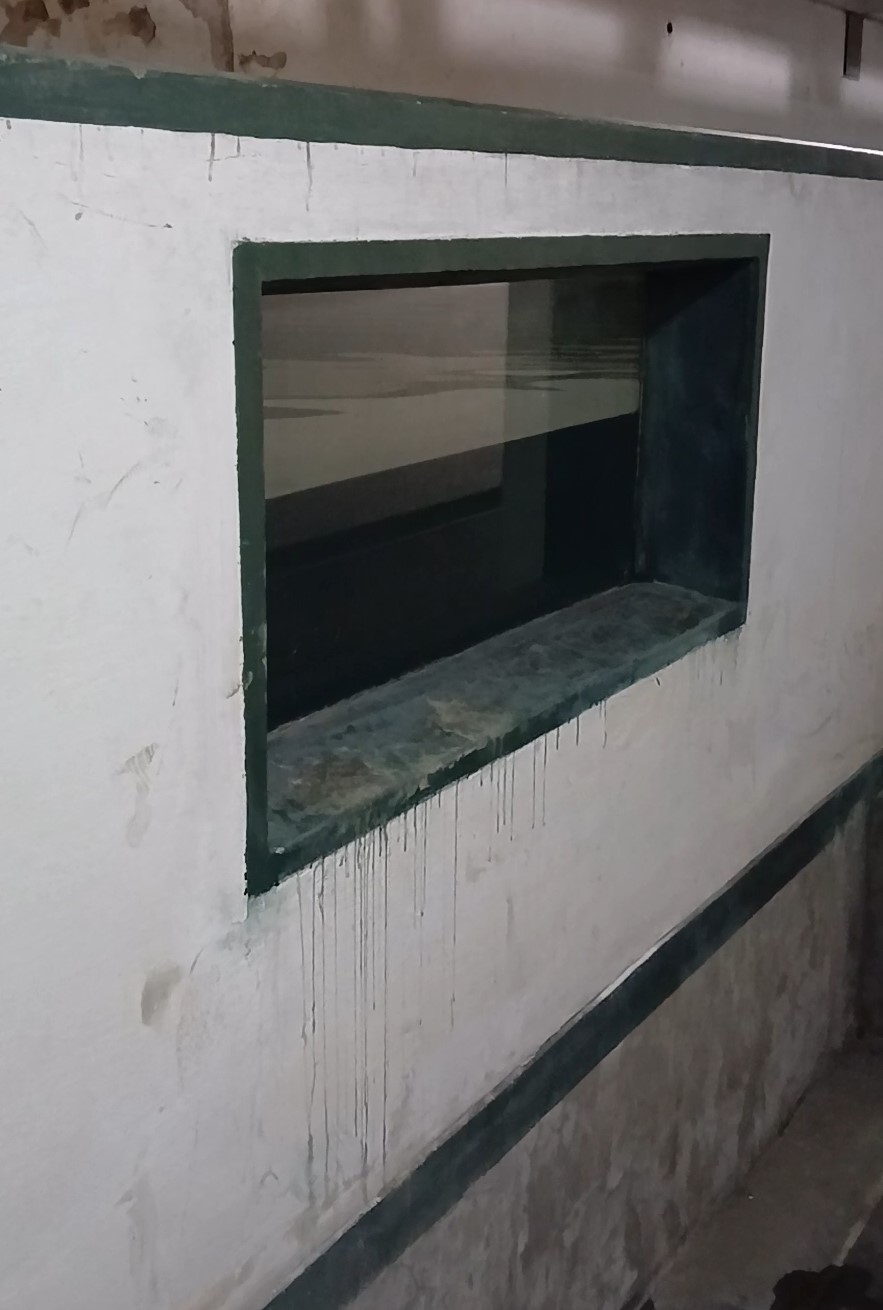
\includegraphics[width=0.2594567\linewidth]{Figures/16_06_2025/Ventana}
	\caption{Ventana al costado del canal.}
	\label{fig:ventana}
\end{figure}

